\chapter{Modèle mathématique}
La modélisation de ce problème a déjà été faite avant ce projet, mais je la remets ici pour assurer la complétude du rapport.

\section{Notions}
Le tableau\ref{fig:var} est un récapitulatif des notions du problème.
\begin{figure}[!htbp]
	\centering
		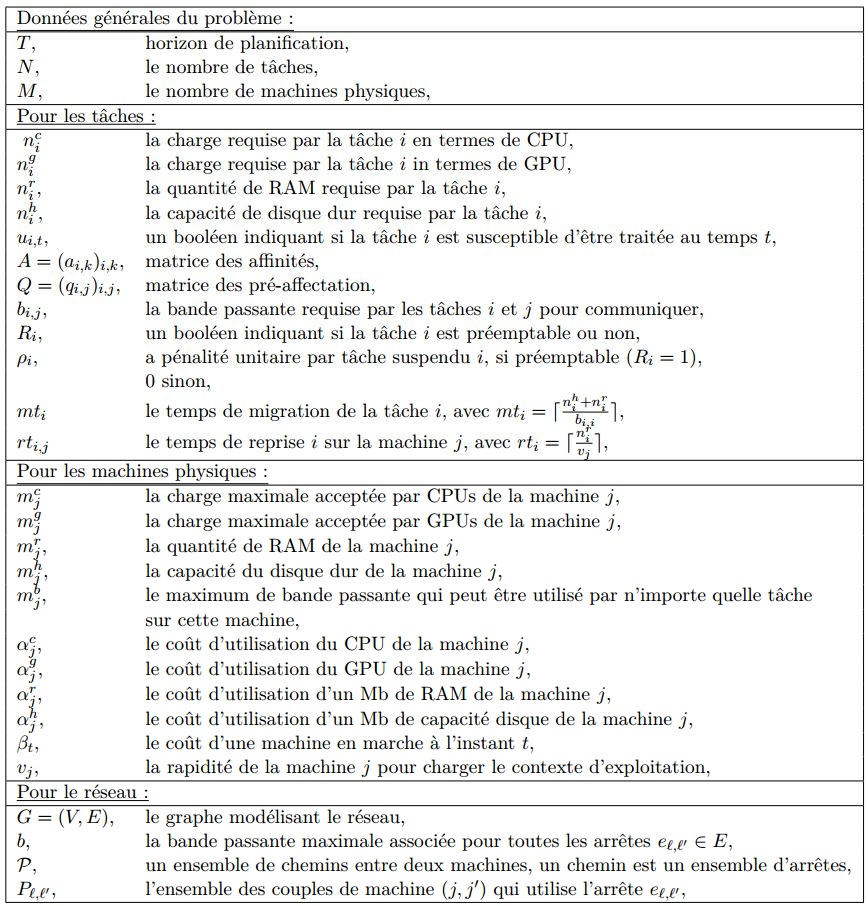
\includegraphics[scale=0.8]{pics/var.jpg}
	\caption{Tableau des variables}
	\label{fig:var}
\end{figure}
\section{Objectifs}
La variable de décision du problème est la suivante qui représente l'ordonnancement en sortie.
$$x_{i,t}^{j}=
\left\{ \begin{array}{rl}
			 1 &\mbox{ si la tâche $i$ est traitée sur la machine $j$ dans l'intervalle $[t, t+1]$} \\
			 0 &\mbox{ sinon}
       \end{array} \right.$$
On définit aussi un ensemble de variables supplémentaires suivantes:
\begin{itemize}
	\item $y_{i,i\prime,t}^{j, j\prime} = 1$ si les deux tâches $i$ et $i\prime$ sont exécutées respectivement sur les machines $j$ et $j\prime$ à l'instant $t$ et ont besoin de communiquer sur le réseau. Au cas de la migration de tâche $i$ de la machine $j$ vers la machine $j\prime$, $y_{i,i,t}^{j, j\prime} = 1$. Dans les autres cas, on a $y_{i,i\prime,t}^{j, j\prime} = 0$.
	\item $z_{t,j} = 1$ si à l'instant $t$ la machine est en état allumé, c'est-à-dire elle exécute au moins une tâche en ce moment.
	\item $z_t$ est le nombre de machines en marche à l'instant $t$.
	\item $d_{i,t}$ est la durée des opérations de reconfiguration de la tâche $i$ à l'instant $t$. Ca peut être la durée d'une opération de $resume$ commançant à $t$ ou bien la durée d'une opération de migration terminant à $t$.
\end{itemize}	
%\clearpage
Maitenant avec les variables et les notions déclarées avant, voici les fonctions objectifs à minimiser.
%\vspace*{-.4cm}
\begin{eqnarray*}
TC &=& \sum_{t=1}^{T}\sum_{i=1}^{N}\sum_{j=1}^{M}{x_{i,t}^{j}(\alpha_j^cn_i^c + \alpha_j^gn_i^g + \alpha_j^hn_i^h + \alpha_j^rn_i^r)} \\
&+&  \sum_{t=1}^{T}\sum_{i=1}^{N}\sum_{j,k=1; k\neq j}^{M}{y_{i,i,t}^{j,k}(\alpha_k^hn_i^h + \alpha_k^rn_i^r)} + \sum_{t=1}^{T}\sum_{i=1}^{N}(1 - \sum_{j=1}^{M}x_{i,t}^{j})\rho_iu_{i,t} +  \sum_{t=1}^{T}{\beta_tz_t}\\
RE &=& \sum_{i=1}^{N}\sum_{t=1}^{T}d_{i,t}
\end{eqnarray*}
%\vspace*{-.4cm}
%\clearpage
\section{Contraintes}
\begin{align} 
 &\sum_{i=1}^{N}{n_i^cx_{i,t}^j} \leq m_j^c  &&\forall t=1,\ldots,T; \nonumber \\
 & &&\forall j=1, \ldots, M     \\
 &\sum_{i=1}^{N}{n_i^gx_{i,t}^j} \leq m_j^g  
  &&\forall t=1,\ldots,T; \nonumber \\
 & &&\forall j=1, \ldots, M        \\                
 &\sum_{i=1}^{N}{n_i^hx_{i,t}^j} + \sum_{j,k=1; k\neq j}^M{n_i^hy_{i,i,t}^{j,k}} \leq m_j^h 
   &&\forall t=1,\ldots,T; \nonumber  \\
  & &&\forall j=1, \ldots, M                   \\    
 &\sum_{i=1}^{N}{n_i^rx_{i,t}^j} + \sum_{j,k=1; k\neq j}^M{n_i^ry_{i,i,t}^{j,k}} \leq m_j^r 
   &&\forall  t=1,\ldots,T; \nonumber \\
  & &&\forall j=1, \ldots, M \\
  %E
  &y_{i,i\prime,t}^{j,j\prime} \geq x_{i,t}^j + x_{i\prime,t}^{j\prime} - 1 
   &&\forall t=1,\ldots,T; \forall i=1, \ldots, N;    \nonumber \\
  & &&\forall i\prime=i+1,\ldots,N dont a_i\prime = 1;  \nonumber \\
  & &&\forall j=1, \ldots, M;  \forall j\prime=j+1, \ldots, M \\
  %F
  &y_{i,i,t}^{j,j\prime} \geq (x_{i,t_1}^j - \sum_{k=1}^M\sum_{t\prime=t_1+1}^{t_2-1}x_{i,t\prime}^k + x_{i,t2}^{j\prime} - 1)
   &&\forall t=1,\ldots,T; \forall i=1, \ldots, N;    \nonumber \\
  & &&\forall j,j\prime=1, \ldots, M et j\neq j\prime;  \nonumber \\
  & &&\forall t_1=t, \ldots, Min(t+mt_i, T) \nonumber \\           
  & &&\forall t_2=t_1+1, \ldots, T \\
  %F'
  &mt_i(x_{i,t}^j - \sum_{k=1}^M\sum_{t\prime=t+1}^{t_1-1}x_{i,t\prime}^k + x_{i,t_1}^{j\prime} - 1) \leq \sum_{t\prime=max(t+1-mt_i, 0)}^tx_{i,t}^j 
   &&\forall t=1,\ldots,T; \forall i=1, \ldots, N;    \nonumber \\
  & &&\forall j,j\prime=1, \ldots, M et j\neq j\prime;  \nonumber \\
  & &&\forall t_1=t+1, \ldots, T \\
  %G
  &\sum_{j=1}^Mx_{i,t}^j = u_{i,t}  &&\forall i=1, \ldots, N, dont R_i=0; \nonumber \\
  & &&\forall t=1,\ldots,T \\
  %H
  &\sum_{j=1}^Mx_{i,t}^j \leq u_{i,t} 
   &&\forall i=1, \ldots, N, dont R_i=1; \nonumber \\
  & &&\forall t=1,\ldots,T \\
  %I
  &x_{i,t}^j \leq u_{i,t}q_{i,j} 
   &&\forall t=1,\ldots,T; \forall i=1, \ldots, N;    \nonumber \\
  & &&\forall j=1, \ldots, M \\
  %J
  &\sum_{(j,j\prime)\in P_{l,l\prime}, j<j\prime}(
   \sum_{i,i\prime=1, i<i\prime, a_{i,i\prime}=1}^N b_{i, i\prime}y_{i,i\prime,t}^{j,j\prime}
   + \sum_i^N b_{i, i}(y_{i,i,t}^{j,j\prime} + y_{i,i,t}^{j\prime,j})
  ) \leq b \nonumber \\
  & &&\forall t=1,\ldots,T; \forall e_{l,l\prime}\in E 
\end{align}
\clearpage
\begin{align}
	%K
  &z_{t,j} \geq x_{i,t}^j 
   &&\forall t=1,\ldots,T; \forall i=1, \ldots, N;    \nonumber \\
  & &&\forall j=1, \ldots, M \\  
  %L
  &z_{t} = \sum_{j=1}^Mz_{t,j} &&\forall t=1,\ldots,T \\
  %M
  &x_{i,t_2}^j \leq 1 - x_{i,t_1}^j + x_{i,t_1+1}^j  
   &&\forall i=1, \ldots, N, dont R_i=1;    \nonumber \\
  & &&\forall j=1, \ldots, M;  \nonumber \\
  & &&\forall t_1=1, \ldots, T-rt_{i,j}; \nonumber \\           
  & &&\forall t_2=t_1+1, \ldots, t_1+rt_{i,j} \\
  %N
  &d_{i,t_1} \geq (t_2 - t_1)(x_{i,t_1-1}^j - \sum_{k=1}^M\sum_{t=t_1}^{t_2-1}x_{i,t}^k - 1 + x_{i,t_2}^j)
   &&\forall i=1, \ldots, N, dont R_i=1;    \nonumber \\
  & &&\forall j=1, \ldots, M;  \nonumber \\
  & &&\forall t_1=1, \ldots, (T-rt_{i,j}-1); \nonumber \\           
  & &&\forall t_2=t_1+rt_{i,j}+1, \ldots, T \\
  %O
  &d_{i,t_1} \geq mt_i(x_{i,t_1}^j  + x_{i,t_1+1}^{j\prime} -1)  &&\forall i=1, \ldots, N;    \nonumber \\
  & &&\forall j,k=1, \ldots, M, j\neq k;  \nonumber \\
  & &&\forall t_1=1, \ldots, (T-mt_i-1); \nonumber \\           
  & &&\forall t_2=t_1+mt_i+1, \ldots, T
\end{align}
